%\usepackage{casouso_estilo}
%\chapter{An\'alisis y Dise\~no} % (fold)

\section{Glosario de Términos}

\begin{description}
\item [Usuario o Entidad:] Persona que utiliza el servicio de almacenamiento para guardar archivos en la nube.
\item [Archivo: ] Conjunto de datos almacenados en la memoria de una computadora que puede manejarse con una instrucción única.
\item [Nube: ] Espacio de almacenamiento y procesamiento de datos y archivos ubicado en internet, al que puede acceder el usuario desde cualquier dispositivo. 
\item [Privacidad: ] Capacidad que una organización o individuo tiene para determinar qué datos en un sistema informático pueden ser compartidos con terceros.
\item [Seguridad: ] Conjunto de medidas preventivas y reactivas de las organizaciones o sistemas tecnológicos que permiten resguardar y proteger la información, buscando mantener la confidencialidad, disponibilidad e integridad de datos de la misma.
\item [Duplicación: ] Acción y efecto de duplicar.
\item [Duplicar: ] Repetir exactamente algo, hacer una copia de ello.
\item [Cifrar: ] Escribir un mensaje en clave mediante un sistema de signos formado por números, letras, símbolos, etc.
\item [Descifrar: ] Declarar lo que está escrito en cifra o en caracteres desconocidos, sirviéndose de clave dispuesta para ella, o sin clave, por conjeturas y reglas críticas.
\item [Conjetura: ] Juicio que se forma de algo por indicios u observaciones.
\item [Mensaje: ] Información transmitida.
\item [Algoritmo Criptográfico: ] Es una función matemática usada en los procesos de cifrado y descifrado.Trabaja en combinación con una llave para cifrar y descifrar datos. 
Modifica los datos de un documento con el objeto de alcanzar algunas características de seguridad (autenticación, integridad y confidencialidad).
\item [Clave o Llave: ] Código de signos convenidos para la transmisión de mensajes secretos o privados.
\item [Aritmética Modular: ] Es un sistema aritmético para clases de equivalencia de números enteros llamadas clases de congruencia. 
\item [Función Computacional: ] Funciones que pueden ser calculadas por una máquina de Turing.
\item [Opacidad: ] Cualidad de opaco.
\item [Opaco: ] Oscuro.
\end{description}


\section{Arquitectura del sistema. }
\begin{figure}[H]
\centering
	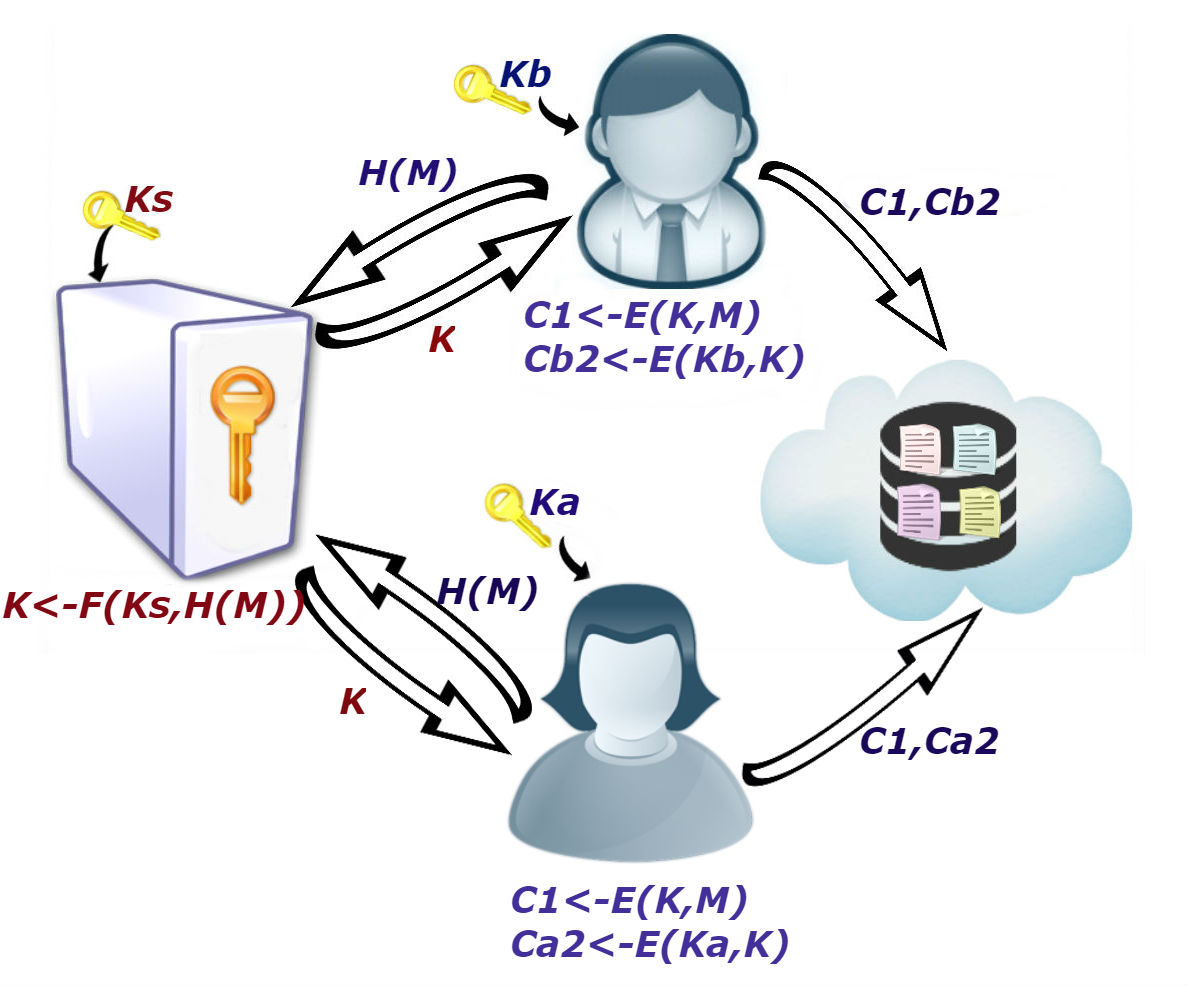
\includegraphics[width=16cm, height=12cm]{./images/Arquitectura.jpg}
	\caption{Arquitectura del sistema.}

\end{figure}

\section{Descripcion de procesos}

\subsubsection{Descripción del proceso subir archivo.}

El proceso inicia cuando el cliente desea subir un archivo nuevo, el cliente debe dar clic en la opción de subir archivo y seleccionar el archivo que desee subir, el sistema va a calcular el hash del archivo elegido, después hará unas operaciones aritméticas con el has para generar una x que se enviara al servidor para que realice una firma a ciegas, y con esta firma que se le regresara al cliente, se va a generar del lado del cliente su llave "k" que será la llave con la cual cifrara el archivo, y así si otro archivo que se quiera subir es igual a este tendrá la misma k y podrá el sistema detectar que son duplicados, también el sistema va a cifrar la llave k por si se le llega a perder al cliente, para poder almacenarlo en la nube el sistema mandara el hash del archivo cifrado para ver si ya está registrado en la base de datos, si es así solo guarda la llave y actualiza la lista de los usuario que comparten el archivo, de lo contrario solicita la llave cifrada y el archivo cifrado para almacenarlos y actualiza su lista de usuario añadiendo un archivo en ella, y por último se le notificará al cliente que su archivo ha sido almacenado.



% - - - - - - - - - - - - - - - - - - - - - - - - -
\subsubsection{Participantes}

\begin{tabular}{ |p{2cm}|p{6cm}|p{6cm}|  }
\hline
\multicolumn{3}{|c|}{  Participantes  } \\
\hline

{ Nombre }  & { Descripción } & { Responsabilidades} \\
\hline
{ Servidor } &  Actor que realiza la firma a ciegas del archivo.  &  
			\begin{itemize}	
				\item Frima a ciegas.

			\end{itemize}   \\ 
\hline
{ Cliente } &   Actor que sube archivos a la Nube.  &  
			\begin{itemize}	
				\item Selecciona archivo a subir.
				\item Genera hash del archivo. 
				\item Calcula la llave k.
				\item Cifra los archivos a subir.
			\end{itemize}   \\ 
\hline
{ Nube } &   Actor que almacena los archivos.  &  
			\begin{itemize}	
				\item Almacena los archivos seleccionados.
				\item Genera lista de usuarios relacionados.
			\end{itemize}   \\ 
\hline
\end{tabular}


\begin{figure}[H]
\centering
	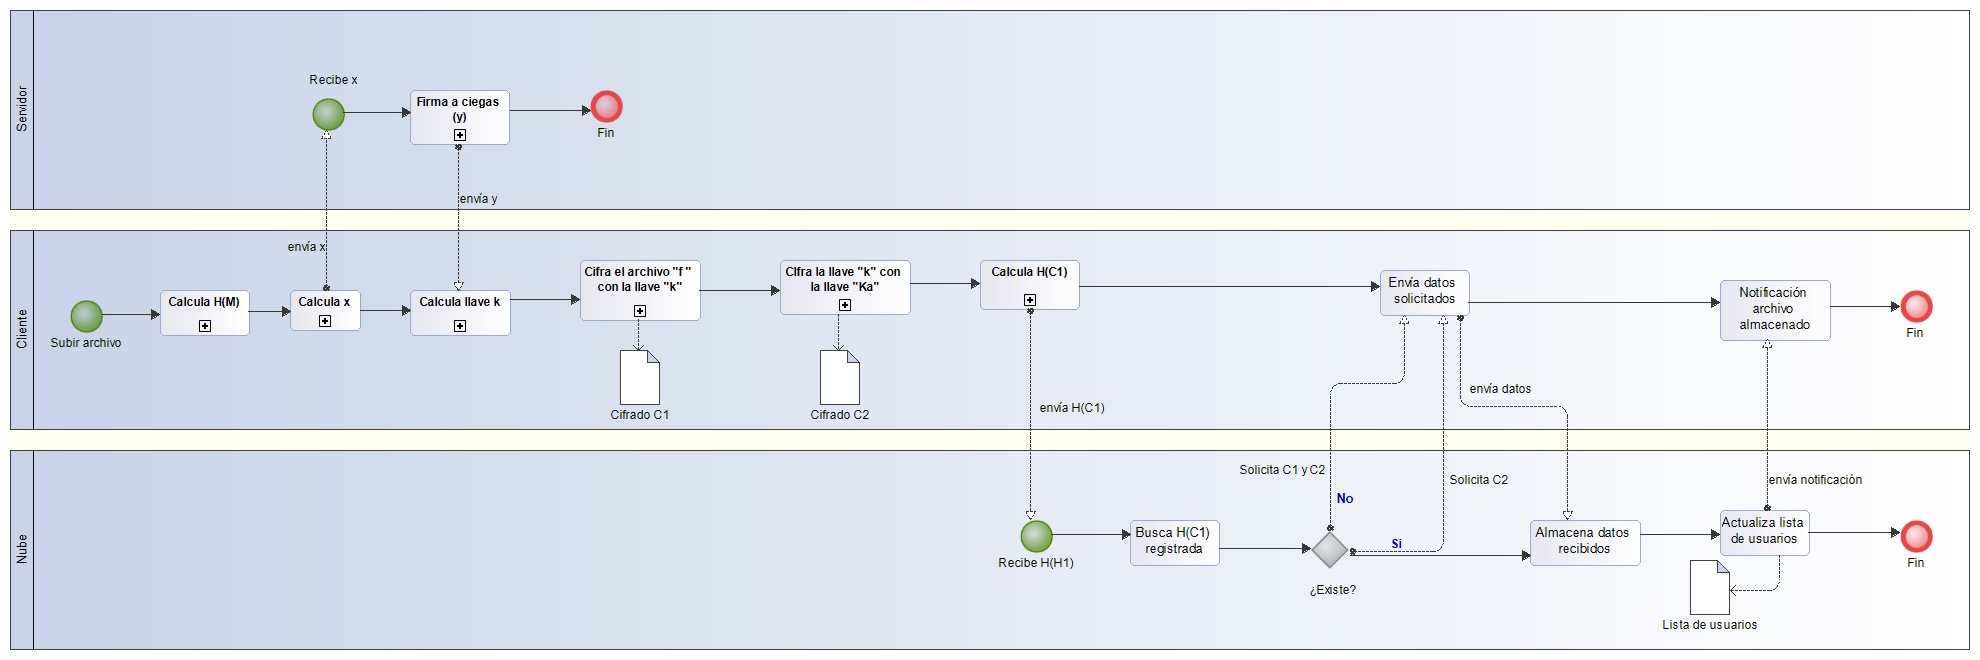
\includegraphics[width=16cm, height=7cm]{./images/BPM_Subir.png}
	\caption{BPMN Subir archivo.}

\end{figure}


\subsubsection{Descripción del proceso Descargar archivo.}

El proceso inicia cuando el cliente desea descargar un archivo, el cliente debe dar clic en la opción de descargar archivo y seleccionar el archivo que desee descargar, el sistema va a mandar el nombre del archivo a la nube para que busque en su base de datos los archivos correspondientes al usuario y nombre del archivo, se le regresaran al cliente y el sistema en el lado del cliente deberá descifrar el archivo C2 que contiene la llave k para poder descifrar el otro archivo C1 donde se encuentra el archivo original, el sistema notificara al cliente que su archivo se ha descargado con éxito y este podrá abrirlo. \\


% - - - - - - - - - - - - - - - - - - - - - - - - -
\subsubsection{Participantes}

\begin{tabular}{ |p{2cm}|p{6cm}|p{6cm}|  }
\hline
\multicolumn{3}{|c|}{  Participantes  } \\
\hline

{ Nombre }  & { Descripción } & { Responsabilidades} \\
\hline
{ Cliente } &   Actor que descarga archivos de la Nube.  &  
			\begin{itemize}	
				\item Selecciona archivo a descargar.
				\item Descifra los archivos descargados.
			\end{itemize}   \\ 
\hline
{ Nube } &   Actor que almacena los archivos.  &  
			\begin{itemize}	
				\item Almacena los archivos seleccionados.
				\item Genera lista de usuarios relacionados.
				\item Enviar los archivos a descargar.
			\end{itemize}   \\ 
\hline
\end{tabular}

\begin{figure}[H]
\centering
	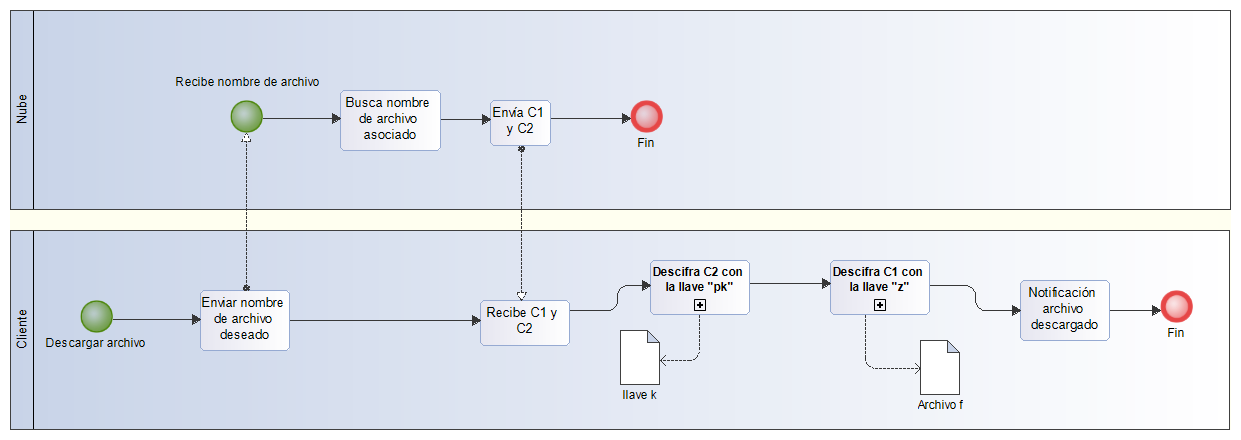
\includegraphics[width=16cm, height=7cm]{./images/BPM_Descargar.png}
	\caption{BPMN Descargar archivo.}

\end{figure}

\vspace{3cm}
\subsubsection{Descripción del proceso eliminar archivo.}

El proceso inicia cuando el cliente desea eliminar un archivo nuevo, el cliente debe dar clic en la opción de eliminar archivo y seleccionar el archivo que desee eliminar, el sistema va a enviar el nombre del archivo a la nube donde este buscara en su base de datos los archivos que corresponden al usuario y nombre del archivo, los va a eliminar de su base de datos y actualizara su lista de usuarios eliminado de ella los datos del archivo y usuario que coinciden con el archivo eliminado, se le enviara una notificación al cliente que su archivo ha sido eliminado con éxito de la nube.\\



% - - - - - - - - - - - - - - - - - - - - - - - - -
\subsubsection{Participantes}

\begin{tabular}{ |p{2cm}|p{6cm}|p{6cm}|  }
\hline
\multicolumn{3}{|c|}{  Participantes  } \\
\hline

{ Nombre }  & { Descripción } & { Responsabilidades} \\
\hline
{ Cliente } &   Actor que elimina archivos de la Nube.  &  
			\begin{itemize}	
				\item Selecciona archivo a elminar.
			\end{itemize}   \\ 
\hline
{ Nube } &   Actor que almacena los archivos.  &  
			\begin{itemize}	
				\item Elimina los archivos seleccionados.
				\item Genera lista de usuarios relacionados.
			\end{itemize}   \\ 
\hline
\end{tabular}

\begin{figure}[H]
\centering
	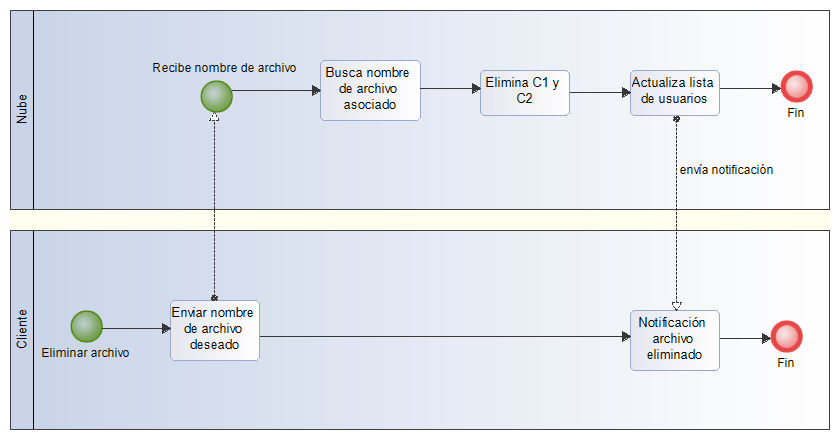
\includegraphics[width=16cm, height=7cm]{./images/BPM_Eliminar.png}
	\caption{BPMN Eliminar archivo.}

\end{figure} 

\newpage

\section{Requerimientos Funcionales. }

\begin{table}[htb]
\centering
\begin{tabular}{| p{2cm} |  p{13.5cm} |}
\hline
\multicolumn{2}{|c|}{\textbf{Servidor de Llaves}} \\ \hline
\textbf{ID} &  \textbf{Descripción} \\
\hline \hline
RF – SLL1 & El sistema permitirá la generación de llaves de usuario a través de una clave secreta (Kg) propia del servidor de llaves. \\ \hline
%RF – SLL2 & El sistema debe gestionar 3 estados en el servidor de llaves: Generación, Cambios y Eliminación de llaves de usuarios para manipular un archivo. \\ \hline
%RF – SLL3 & El sistema comenzará la creación de una llave (K) cuando el usuario solicite la carga de un archivo a almacenar. \\ \hline
%RF – SLL4 & El sistema deberá enviar al cliente la llave generada en el servidor de llaves (K) del archivo que el usuario solicitó carga al servicio de almacenamiento. \\ \hline
RF – SLL2 & El sistema permitirá la firma a ciegas (y) de cualquier archivo que se desee almacenar. \\ \hline
%RF – SLL3 & El sistema actualizará la base de datos del servidor de llaves cada vez que una nueva firma (y) sea generada dentro de éste. \\ \hline
%RF – SLL7 & El sistema detectará mediante la función hash del archivo [H(F)] si se le ha generado anteriormente una llave (K), si ésta existe en la base de datos se procederá a enviarla al usuario que la solicita. \\ \hline
%RF – SLL8 & El sistema modificará la llave (K) para un archivo cuando este sea modificado por el propietario del archivo (F). \\ \hline
%RF – SLL9 & El sistema eliminará la llave (K) para un archivo cuando este sea eliminado del servicio de almacenamiento por el usuario. \\ \hline
\end{tabular}
\caption{Requerimientos funcionales del servidor de llaves}
\label{Servidor de Llaves }
\end{table}


\begin{table}[htb]
\centering
\begin{tabular}{| p{2cm} |  p{13.5cm} |}
\hline
\multicolumn{2}{|c|}{\textbf{Cliente}} \\ \hline
\textbf{ID} &  \textbf{Descripción} \\
\hline \hline
RF – CL1 & El sistema permitirá al usuario gestionar archivos: Subir, Descargar, Eliminar \\ \hline
%RF – CL2 & El sistema permitirá al usuario calcular a su archivo (F) una función hash [H(F)] cuando dicho usuario solicite una nueva carga de éste. \\ \hline
RF – CL2 & El sistema permitirá al usuario subir un archivo (F) cifrado al servicio de almacenamiento  \\ \hline
%RF – CL4 & El sistema entregará al cliente la llave (K) generada en el servidor de llaves del archivo (F) que el usuario solicitó cargar al servicio de almacenamiento.  \\ \hline
%RF – CL5 & El sistema mandará a cifrar la llave (K) obtenida del servidor de llaves junto con el archivo (F) que el usuario desea cargar al servicio de almacenamiento. \\ \hline
%RF – CL6 & El sistema obtendrá el cifrado C1 correspondiente al archivo original (F)  y lo mandará al cliente, cifrado que el usuario cargará al servicio de almacenamiento.  \\ \hline
%RF – CL7  & El sistema calculará al cifrado C1 una función hash [H(C1)] \\ \hline
%RF – CL8  & El sistema mandará a cifrar la llave secreta (Ka) del usuario junto con la llave (K) obtenida del servidor de llaves del archivo (F) que éste usuario desea cargar al servicio de almacenamiento. \\ \hline
%RF – CL9  & El sistema obtendrá el cifrado C2 correspondiente a la llave secreta (Ka) del usuario y lo mandará al cliente, cifrado que el usuario cargará al servicio de almacenamiento. \\ \hline
%RF – CL10 & El sistema enviará [H(C1)] hacia el servicio de almacenamiento para su evaluación. \\ \hline
RF – CL3 & El sistema permitirá al usuario descargar un archivo (F) descifrado elejido de su lista de archivos en el servicio de almacenamiento\\ \hline
%RF – CL12 & El sistema notificará al usuario el estatus final de la gestión de sus archivos en el servicio de almacenamiento.  \\ \hline
RF – CL4 &El sistema permitirá al usuario eliminar un archivo (F) cuando el usuario elige alguno de su lista de archivos cargados en el servicio de almacenamiento  \\ \hline
%RF – CL14 & El sistema entregará al cliente el cifrado C1 correspondiente al archivo (F) que el usuario eligió y el cifrado C2 que corresponde a la llave (K) del mismo archivo. \\ \hline
%RF – CL15 & El sistema enviará desde el cliente al módulo cifrador la llave secreta (Ka) del usuario junto con el cifrado C1 y C2.  \\ \hline
%RF – CL16 & El sistema obtendrá el archivo original (F) que solicitó el usuario para la descarga.  \\ \hline
RF – CL5 & El sistema generará la llave (K) correspondiente a la firma (Y) que envió el servidor de llaves  \\ \hline
%RF – CL18 & El sistema enviará al servidor de almacenamiento el nombre del archivo (F) que el usuario solicite eliminar.  \\ \hline
%RF – MC1 & El sistema recibirá en el modulo cifrador la llave (K) obtenida del servidor de llaves junto con el archivo (F) que el usuario desea cargar. \\ \hline
RF – CL6 & El sistema cifrará el archivo (F) que el usuario a solicitado \\ \hline
%RF – MC3 & El sistema enviará al cliente el archivo C1 obtenido en el módulo cifrador. \\ \hline
%RF – MC4 & El sistema recibirá en el módulo cifrador la llave secreta (Ka) del usuario junto con la llave (K) obtenida del servidor de llaves del archivo (F) que éste usuario desea cargar \\ \hline
RF – CL7 & El sistema descifrará el archivo (F) que el usuario a solicitado  \\ \hline
%RF – MC6 & El sistema enviará al cliente el archivo C2 obtenido en el módulo cifrador. \\ \hline
%RF – MC7 & El sistema recibirá en el modulo cifrador la llave secreta (Ka) junto con el cifrado C1 y el cifrado C2 que el usuario solicite descargar.\\ \hline
%RF – MC9 & El sistema descifrará el C2 junto con la llave (K) que el usuario a solicitado descargar y generará el archivo original (F).\\ \hline
\end{tabular}
\caption{Requerimientos funcionales del cliente}
\label{Cliente }
\end{table}


\begin{table}[htb]
\centering
\begin{tabular}{| p{2cm} |  p{13.5cm} |}
\hline
\multicolumn{2}{|c|}{\textbf{Servicio de almacenamiento (Nube)}} \\ \hline
\textbf{ID} &  \textbf{Descripción} \\
\hline \hline
RF – SA1 & El sistema permitirá al servicio de almacenamiento gestionar archivos: Almacenar, Descargar y Eliminar.\\ \hline
%RF – SA2 & El sistema creará una base de datos con los cifrados que cada usuario tenga registrados dentro del servicio de almacenamiento.\\ \hline
RF – SA2 & El sistema permitirá al servicio de almacenamiento guardar cualquier cifrado que el usuario solicite cargar. \\ \hline
RF – SA3 & El sistema permitirá al servicio de almacenamiento descargar cualquier cifrado que el usuario tenga en su lista de archivos. \\ \hline
RF – SA4 & El sistema permitirá al servicio de almacenamiento eliminar cualquier cifrado que el usuario tenga en su lista de archivos. \\ \hline
%RF – SA6 & El sistema actualizará dentro de la base de datos del servicio de almacenamiento, la lista de archivos (F) que el usuario a gestionado dentro de éste. \\ \hline
%RF – SA7 & El sistema entregará [H(C1)] generado por el cliente al servicio de almacenamiento \\ \hline
%RF – SA8 & El sistema almacenará en una base de datos dentro del servicio de almacenamiento a [H(C1)] asociando al cliente que lo envió. \\ \hline
%RF – SA9 & El sistema corroborará la existencia [H(C1)] dentro de la base de datos, si existe procederá al RF – SA6,  si no procederá al RF – SA3\\ \hline
%RF – SA10 & El sistema entregará al servidor de almacenamiento el nombre del archivo (F) que el usuario solicite eliminar.\\ \hline
%RF – SA11 & El sistema eliminará el nombre del archivo (F) de la lista de archivos que el usuario tiene registrados en la base de datos del servidor de almacenamiento. \\ \hline
%RF – SA12 & El sistema enviará una notificación al cliente con el estatus de cada gestión hecha por el usuario sobre sus archivos. \\ \hline
%RF – SA13 & El sistema recibirá el nombre del archivo (F) que el usuario solicita descargar.\\ \hline
%RF – SA14 & El sistema buscará el nombre del archivo (F) en la base de datos de los cifrados que tiene el usuario registrados en el servicio de almacenamiento.\\ \hline
%RF – SA15 & El sistema enviará al cliente el archivo C1 correspondiente al archivo (F) que el usuario eligió y el cifrado C2 que corresponde a la llave (K) del mismo archivo. \\ \hline
\end{tabular}
\caption{Requerimientos funcionales del Servicio de almacenamiento (Nube)}
\label{Servicio de almacenamiento (Nube) }
\end{table}

\vspace{9cm}
\section{Requerimientos No Funcionales }
\begin{longtable}{| p{1.5cm} | p{3cm} | p{11cm} |}

% aquí añadimos el encabezado de la primera hoja.
\hline
\multicolumn{3}{|c|}{\textbf{Requerimientos No Funcionales}} \\ \hline
\textbf{ID} &  \textbf{Atributo} & \textbf{Descripción}\\
\hline \hline
\endfirsthead

% aquí añadimos el encabezado del resto de hojas.
\hline
\textbf{ID} &  \textbf{Atributo} & \textbf{Descripción}\\
\hline \hline
\endhead

% aquí añadimos el fondo de todas las hojas, excepto de la última.
\multicolumn{3}{|c|}{Sigue en la página siguiente.}
\endfoot

% aquí añadimos el fondo de la última hoja.
\endlastfoot

% aquí añadimos el cuerpo de la tabla.
RNF1 & Eficiencia &  \begin{itemize} 
   \item El servidor de llaves tendrá la capacidad de realizar 1000 peticiones de gestión de almacenamiento de archivos por segundo. 
   \item El sistema podrá funcionar de forma correcta con usuarios conectados de manera concurrente. 
   \item Los archivos que sean gestionados dentro del servidor de almacenamiento, deben ser actualizados en la base datos y la visualización de cada cliente de manera casi inmediata. 
  \end{itemize}
\\ \hline

RNF2 & Fiabilidad &  \begin{itemize} 
  \item La pérdida de consultas en el servidor de llaves es menor a 3 veces el máximo de consultas realizadas. 
   \item Los archivos almacenados en el servidor de almacenamiento deben ser recuperados por el usuario al instante en que este lo solicite. 
   \item El tiempo de latencia que existe entre el servidor de llaves y el cleinte será de máximo 118ms. 
 \end{itemize}
\\ \hline

RNF3 & Seguridad & \begin{itemize} 
    \item El sistema almacenará los datos de los usuarios y sus contraseñas en una base de datos MySQL, dichos datos serán modificados mínimo 2  veces al año.  
   \item Se autenticarán los clientes antes de comenzar el proceso de generación de llaves de archivo. 
   \item El servidor de llaves firmará claves para un sólo mensaje a la vez sin saber el contenido de éste. 
   \item El inicio de sesión de usuarios estará protegido en un canal seguro utilizando almoritmos criptográficos. 
   \item Las funciones hash de archivos a almacenar utilizarán la función criptográfica SHA-(256)
 \end{itemize}

\\ \hline 
RNF4 & Mantenibilidad & \begin{itemize}
   \item Cuaquier nuevo requerimiento funcional o no funcional tendrá que ser analizado y diseñado para poder cuantificar las implicaciones que este tendrá sobre el funcionamiento del sistema. 
   \item El sistema contará con un plan de pruebas que facilitará la identificación de posibles fallas existentes en el funcionamiento de este. 
 \end{itemize}
\\ \hline
\caption{Requerimientos no funcionales del sistema}
\label{Servidor de Llaves }
\end{longtable}

\section{Reglas de Negocio}

\begin{BussinesRule}{RN1}{Datos requeridos} 
	\BRitem[Descripción:]  El usuario debe ingresar toda la información marcada como requerida en el modelo conceptual del negocio.
	\BRitem[Tipo:] Restricción de operación.	
\end{BussinesRule}

\begin{BussinesRule}{RN2}{Datos correctos} 
	\BRitem[Descripción:] La información que el usuario proporcione, debe ser del tipo y longitud definida en el modelo conceptual del negocio.
	\BRitem[Tipo:] Restricción de operación.	
\end{BussinesRule}

\begin{BussinesRule}{RN3}{Unicidad de elementos} 
	\BRitem[Descripción:] Hay ciertos elementos que no pueden repetirse, ya sea por ser idénticos o por coincidir en uno o más datos. Esto se define como dato único en la tabla de atributos del modelo conceptual del negocio para cada entidad.
	\BRitem[Tipo:] Restricción de operación.	
\end{BussinesRule}

\begin{BussinesRule}{RN4}{Usuario registrado} 
	\BRitem[Descripción:] El usuarios debe tener una cuenta activa en el sistema.
	\BRitem[Tipo:] Hecho
\end{BussinesRule}

\section{Especificación de Plataforma}


%\textbf{Servidor web}
%\begin{enumerate}
%\item \textbf{Hardware}
%\begin{itemize}
%\item Procesador: Intel Xeon 1220
%\item RAM: 4 GB DDR3 1600 MHz
%\end{itemize}
%\item \textbf{Software}
%\begin{itemize}
%\item Sistema operativo: Debian 8 Jessie 64 bits
%\item Servidor web: Apache 2
%\begin{itemize}
%\item Módulo PHP 5 con conector para MongoDB
%\end{itemize}
%\item Servidor de base de datos: MongoDB 3.2
%\end{itemize}
%\item \textbf{Red}
%\begin{itemize}
%\item Conexión a internet cableada de 20 Mb/s
%\end{itemize}
%\end{enumerate}

\textbf{Estación de trabajo y computadores personales}
\begin{enumerate}
\item \textbf{Hardware}
\begin{itemize}
\item Procesador: Intel Celeron N2840 o superior
\item RAM: 2 GB o superior
\end{itemize}
\item \textbf{Software}
\begin{itemize}
\item Navegador Web: Chrome 24, Firefox 24, Internet Explorer 10, Safari 7 o superior.
\begin{itemize}
\item Soporte para cookies
\end{itemize}
\end{itemize}

\item \textbf{Red}
\begin{itemize}
\item Conexión a internet de 2 Mb/s
\end{itemize}

\end{enumerate}

\newpage

\section{Casos de Uso}

\begin{figure}[htbp!]
		\centering
			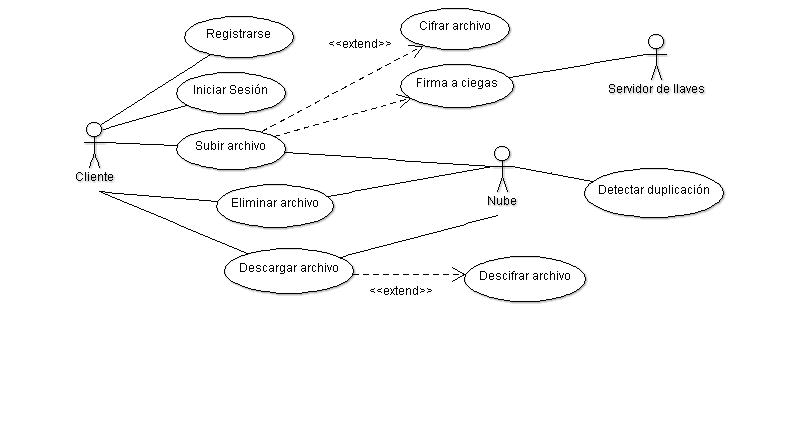
\includegraphics[width=1\textwidth]{images/CasosDeUso}
		\caption{Diagrama de Casos de Uso del sistema.}
	\end{figure}